\let\negmedspace\undefined
\let\negthickspace\undefined
\documentclass[journal]{IEEEtran}
\usepackage[a4paper, margin=10mm, onecolumn]{geometry}
%\usepackage{lmodern} % Ensure lmodern is loaded for pdflatex
\usepackage{tfrupee} % Include tfrupee package

\setlength{\headheight}{1cm} % Set the height of the header box
\setlength{\headsep}{0mm}  % Set the distance between the header box and the top of the text

\usepackage{gvv-book}
\usepackage{gvv}
\usepackage{cite}
\usepackage{amsmath,amssymb,amsfonts,amsthm}
\usepackage{algorithmic}
\usepackage{graphicx}
\usepackage{float}
\usepackage{textcomp}
\usepackage{xcolor}
\usepackage{txfonts}
\usepackage{listings}
\usepackage{enumitem}
\usepackage{mathtools}
\usepackage{gensymb}
\usepackage{comment}
\usepackage[breaklinks=true]{hyperref}
\usepackage{tkz-euclide} 
\usepackage{listings}
% \usepackage{gvv}                                        
\def\inputGnumericTable{}                                 
\usepackage[latin1]{inputenc}                                
\usepackage{color}                                            
\usepackage{array}                                            
\usepackage{longtable}                                       
\usepackage{calc}                                             
\usepackage{multirow}                                         
\usepackage{hhline}                                           
\usepackage{ifthen}                                           
\usepackage{lscape}
\usepackage{tikz}
\usetikzlibrary{patterns}

\begin{document}

\bibliographystyle{IEEEtran}
\vspace{3cm}

\title{1.1.10.31}
\author{ee25btech11063-vejith}

\maketitle
% \maketitle
% \newpage
% \bigskip
{\let\newpage\relax\maketitle}
\renewcommand{\thefigure}{\theenumi}
\renewcommand{\thetable}{\theenumi}
\setlength{\intextsep}{10pt} % Space between text and floats
\textbf{Question}:\\
A vector $\vec{r}$ has magnitude 14 and direction ratios $2$,$3$,$-6$.Find the direction cosines and components of $\vec{r}$, given that $\vec{r}$ makes an acute angle with X axis\\ 
\textbf{Solution}\\
\begin{table}[h!]    
  \centering
  \begin{tabular}{|c|c|c|}
     \hline
     \textbf{Mineral} & \textbf{Modal abundance \brak{\%}} & \textbf{Partition coefficient}\\
     \hline
     Clinopyroxene & $45$ & $0.506$ \\
      \hline
      Orthopyroxene & $40$ & $0.42$ \\
      \hline
      Olivine & $10$ & $0.045$ \\
      \hline
      Plagioclase & $05$ & $0.019$ \\
      \hline
\end{tabular}
  \caption{Variables Used}
  \label{}
\end{table}\\
\begin{align}
     \vec{r}=k\myvec{2\\3\\-6}\\
     \norm{\vec{r}}=\abs{k}\norm{\myvec{2\\3\\-6}}\\
     \norm{\vec{r}}=\abs{k}7\\
     14=\abs{k}7\\
     \abs{k}=2\\
     \implies \vec{r}&=\myvec{4\\6\\-12} 
\end{align}
\hspace*{5cm}\brak{\text{but k=2 not -2 because given that vector r makes  an acute angle with X axis}}\\

The unit  vector in the direction of $\vec{r}$  is
\begin{align}
    \frac{\vec{r}}{\norm{\vec{r}}} &= \frac{1}{14}\myvec{4\\6\\-12} = \myvec{\frac{2}{7}\\\frac{3}{7}\\\frac{-6}{7}}\\
    \end{align}
The component of $\vec{r}$ along X axis =$\vec{r}_X$=\myvec{4\\0\\0}\\
The component of $\vec{r}$ along Y axis =$\vec{r}_Y$=\myvec{0\\6\\0}\\
The component of $\vec{r}$ along Z axis =$\vec{r}_Z$=\myvec{0\\0\\-12}\\
\begin{figure}[h!]
   \centering
   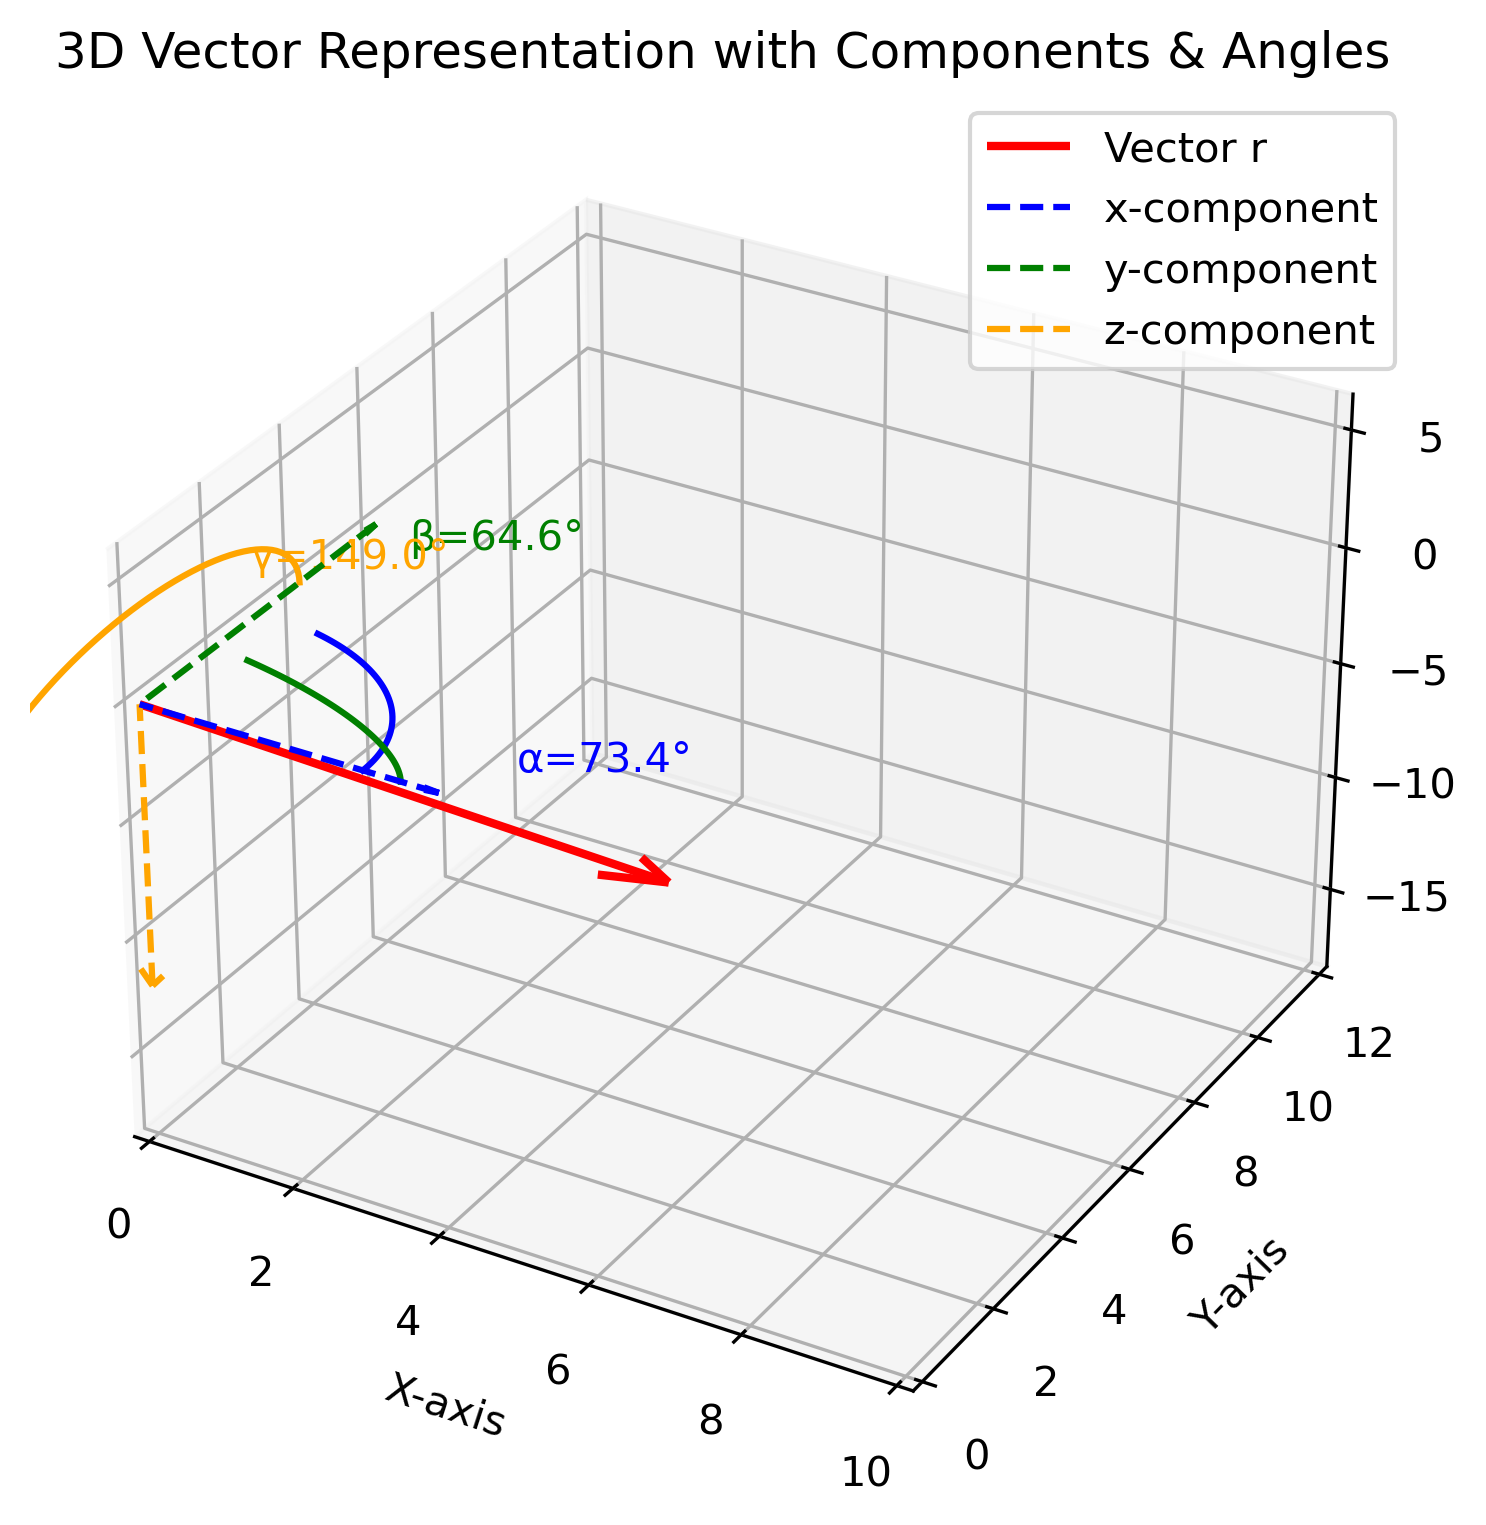
\includegraphics[width=0.5\columnwidth]{figs/01.png}
   \caption{}
   \label{}
\end{figure}
\end{document}
